\documentclass[10pt]{beamer}
\usepackage[utf8]{inputenc}
\usepackage[T1]{fontenc}
%\usepackage[ngerman]{babel}
\usepackage{beamerthemesplit}
\usepackage{color}
%\usepackage{beamerthemeshadow}
\useoutertheme{infolines}
%\usecolortheme{seahorse}

\usepackage{listings}
%\usepackage{bbm}
\usepackage{hyperref}
\usepackage{empheq}
%\usepackage{amsmath}
%\usepackage{amsfonts}
%\usepackage{amssymb}
%\usepackage[dvips]{graphicx}
%\usepackage[dvips]{color}
\title[Räuber-Beute Modell]{Räuber-Beute Modell\\PDE}
\institute[Computerphysik]{Computerphysik WS 18/19}
\date[]{}


\begin{document}

\frame{\titlepage}

\section{Einführung}
\frame
{
  \frametitle{erweitertes Volterra-Lotka Modell}
\begin{eqnarray*}
\frac{\partial u}{\partial t} &=& \delta_1 \Delta u + r u \left(1 - \frac{u}{w} \right) - p v \Psi(k u) \\
\frac{\partial v}{\partial t} &=& \delta_2 \Delta v + q v \Psi(k u) - s v \notag \\
\Psi &:=& \eta \mapsto \tfrac{\eta}{1+\eta} \notag
\end{eqnarray*}
%\vspace{5pt}
\begin{center}
\begin{tabular}{cc}
 Räuber $v(t)$ & Beute $u(t)$\\ 
 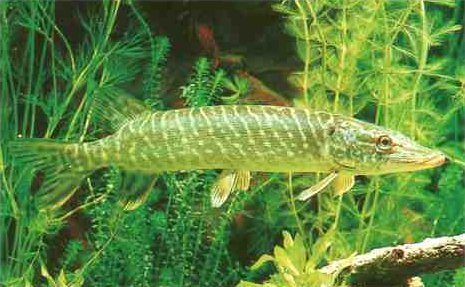
\includegraphics[height=2cm]{img/Hecht.jpg} & 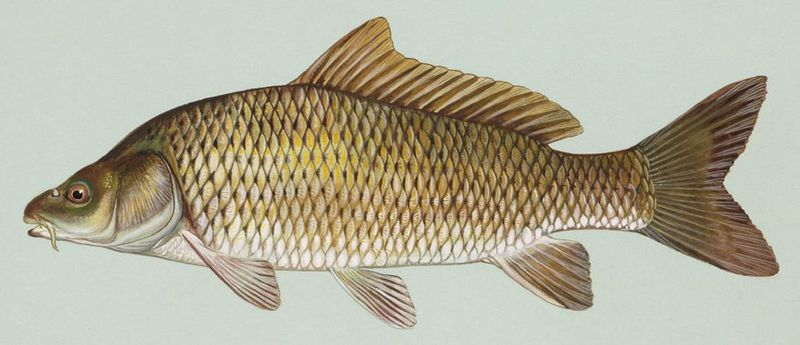
\includegraphics[height=2cm]{img/Karpfen.jpg}\\ 
 Hecht & Karpfen 
\end{tabular}
%bb=14 14 126 84, %,bb=14 14 399 180
\end{center}
\begin{flushright}
 in einem großen See
\end{flushright}
% \begin{flushright}
% \scriptsize{Bilder: Wikipedia}
% \end{flushright}
}




\frame
{
  \frametitle{Randbedingungen}
\begin{eqnarray*}
\frac{\partial u}{\partial t} &=& \delta_1 \Delta u + r u \left(1 - \frac{u}{w} \right) - p v \Psi(k u) \\
\frac{\partial v}{\partial t} &=& \delta_2 \Delta v + q v \Psi(k u) - s v \notag \\
\Psi &:=& \eta \mapsto \tfrac{\eta}{1+\eta} \notag \\
&& \qquad \qquad  \text{in } \Omega = [0, L]^2 \notag \\
\end{eqnarray*}
\vspace{1pt}
\begin{eqnarray*}
  \text{(Neumann)-RB} && \frac{\partial u}{\partial\mathbf n}=\frac{\partial v}{\partial\mathbf n} = 0 \notag\\
  &&\qquad \qquad \text{auf }  \partial\Omega = [0, L]^2 \\
\end{eqnarray*}
}

\section{Diffusionsgleichung}

%Die Lösung kann durch eine Fourier-Reihe $u\left( x,t \right)=\sum_k c_k e^{\mathrm i k x}$ dargestellt werden.\newline\newline

\frame
{
  \frametitle{Diffusionsgleichung}
\begin{equation}
 \frac{\partial u}{\partial t} = D \frac{\partial^2 u}{\partial x^2} = D \Delta u \nonumber
\end{equation}
\\
\textcolor{blue} {Wie sieht die Diffusionsgleichung in diskreter Form aus?}\\
\begin{center}
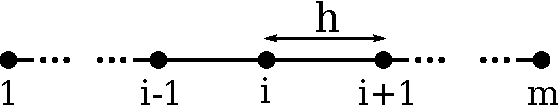
\includegraphics[height=30pt]{img/differencegrid.pdf}
\begin{center}
 \begin{eqnarray*}
  x_i&=& i h \qquad i=0,1,\ldots,\frac{L}{h}\nonumber\\
  t_n&=& n \tau \qquad n=0,1,\ldots
 \end{eqnarray*}
\end{center}
Numerische Lösung $u_j^n$
\end{center}
}

\frame
{
  \frametitle{Diffusionsgleichung}
  \begin{equation}
  \frac{\partial u}{\partial t} = D \frac{\partial^2 u}{\partial x^2} = D \Delta u \nonumber
  \end{equation}
\textcolor{blue} {Wie sieht die Diffusionsgleichung in diskreter Form aus?}\\
Laplace Operator 
\begin{equation}
\Delta_h = \tfrac{1}{h^2}[u_{i+1}^n-2 u_i^n+u_{i-1}^n]
\end{equation}
Euler Methode
\begin{equation*}
\frac{u^{n+1} - u^{n}}{\tau} = F[u^{n}]
\end{equation*}

\begin{equation*}
\boxed{
 \frac{u_j^{n+1}-u_j^n}{\tau}= D\left[\frac{u_{j+1}^n-2 u_j^n+u_{j-1}^n}{h^2}\right]\nonumber
}
\end{equation*}
}

\frame
{
  \frametitle{(Von Neumann) Stabilitätsanalyse}
\begin{equation*}
 \frac{u_j^{n+1}-u_j^n}{\tau}= D\left[\frac{u_{j+1}^n-2 u_j^n+u_{j-1}^n}{h^2}\right]
\end{equation*}\newline
\textcolor{blue}{ Wahl von $\tau$? }
\newline
Stabilität $||u^{n}|| < const$ 
\newline\newline

Fourier-Reihe $u_j^n=\sum_k c_k^n e^{\mathrm i k h j}$; $k$ ist die reele Wellenzahl\newline
komplexer Amplifikationsfaktor $\frac{c_k^{n+1}}{c_k^n}=\xi$\newline

Die Lösung ist stabil für $\mid \xi \mid \leq 1$.\newline\newline
\textcolor{blue} {Was folgt daraus für $\Delta t$ und $\Delta x$?}
\begin{equation*}
|\xi| = \boxed{
\frac{2 D \tau}{h^2}\leq 1
}
\end{equation*}
}

\begin{frame}{Instabilität}
\begin{center}
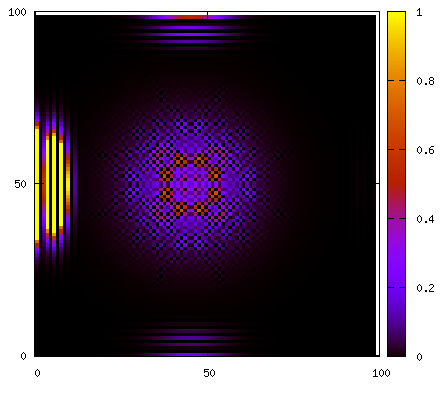
\includegraphics[width=8cm]{img/boom.png}
\end{center}
\end{frame}


\frame
{
\frametitle{2d Laplaceoperator}

\begin{equation}
(\Delta_h u)_{i,j} = \frac{1}{h^2} \left[ -4 u_{i,j} + u_{i-1,j} + u_{i,j-1} + u_{i+1,j} + u_{i,j+1} \right]\nonumber
\end{equation}
\begin{center}
 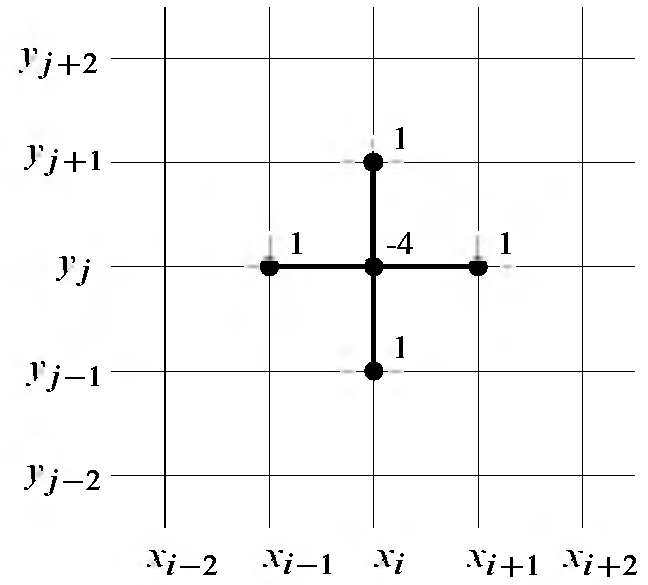
\includegraphics[scale=0.25]{img/gitter3.png}
\end{center}
\textcolor{blue} {Wie kann man den Laplaceoperator am Rand auswerten?}
}


\frame
{
\frametitle{Laplaceoperator am Rand}

\begin{equation}
(\Delta_h u)_{i,j} = \frac{1}{h^2} \left[ -4 u_{i,j} + u_{i-1,j} + u_{i,j-1} + u_{i+1,j} + u_{i,j+1} \right]\nonumber
\end{equation}
von Neumann Randbedingung: $\frac{1}{h} \left[u_{0,j} - u_{-1,j}\right]=0$

\begin{center}
 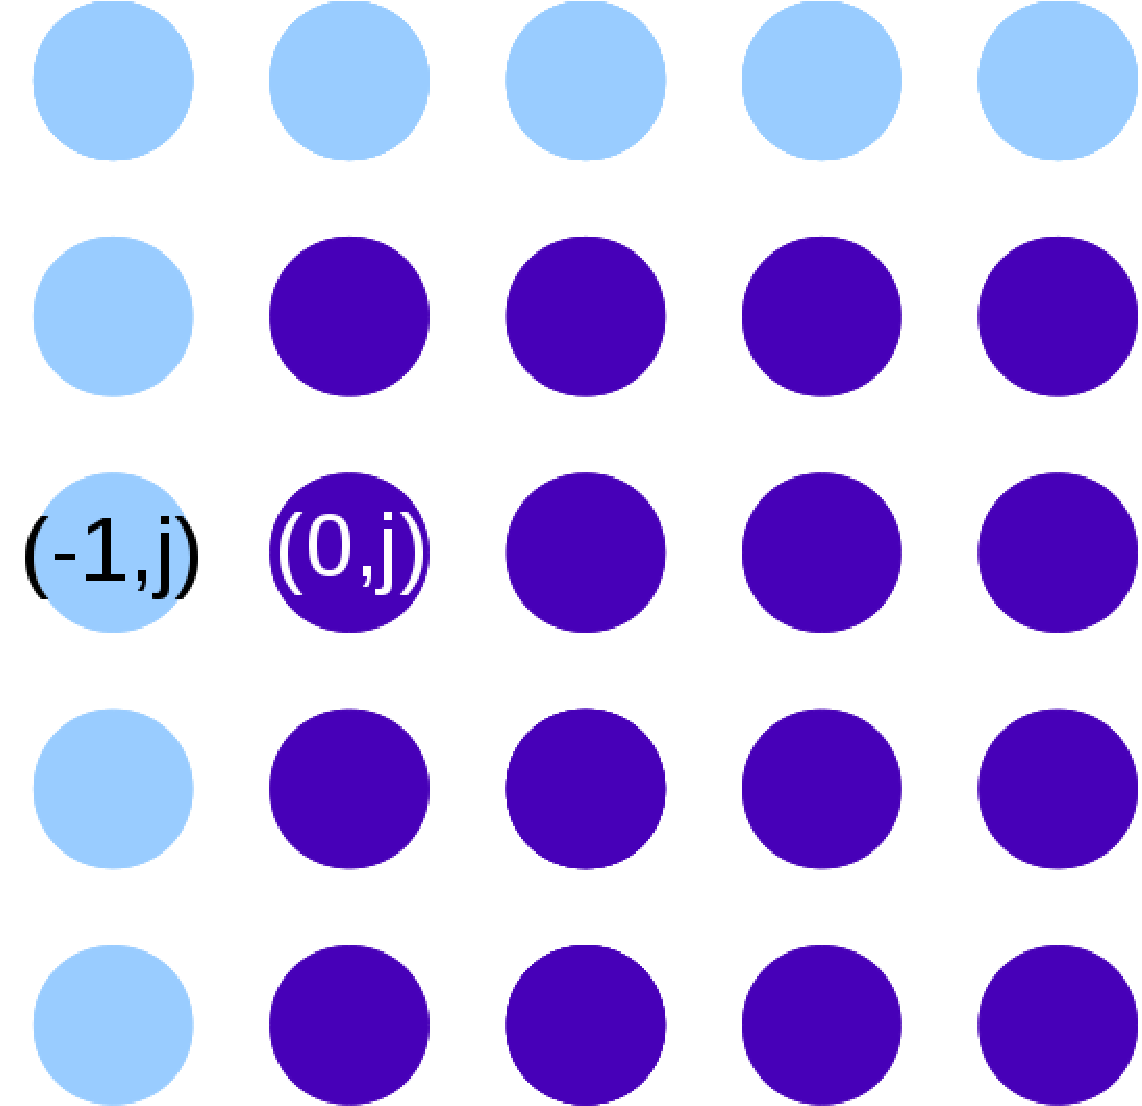
\includegraphics[scale=0.25]{img/Gitter2.pdf} $\quad\Rightarrow u_{-1,j}$ kann eliminiert werden.
\end{center}
durch ``Geisterpunkte'' oder Fallunterscheidung.
}


\begin{frame}{Speicherlayout}
\begin{center}
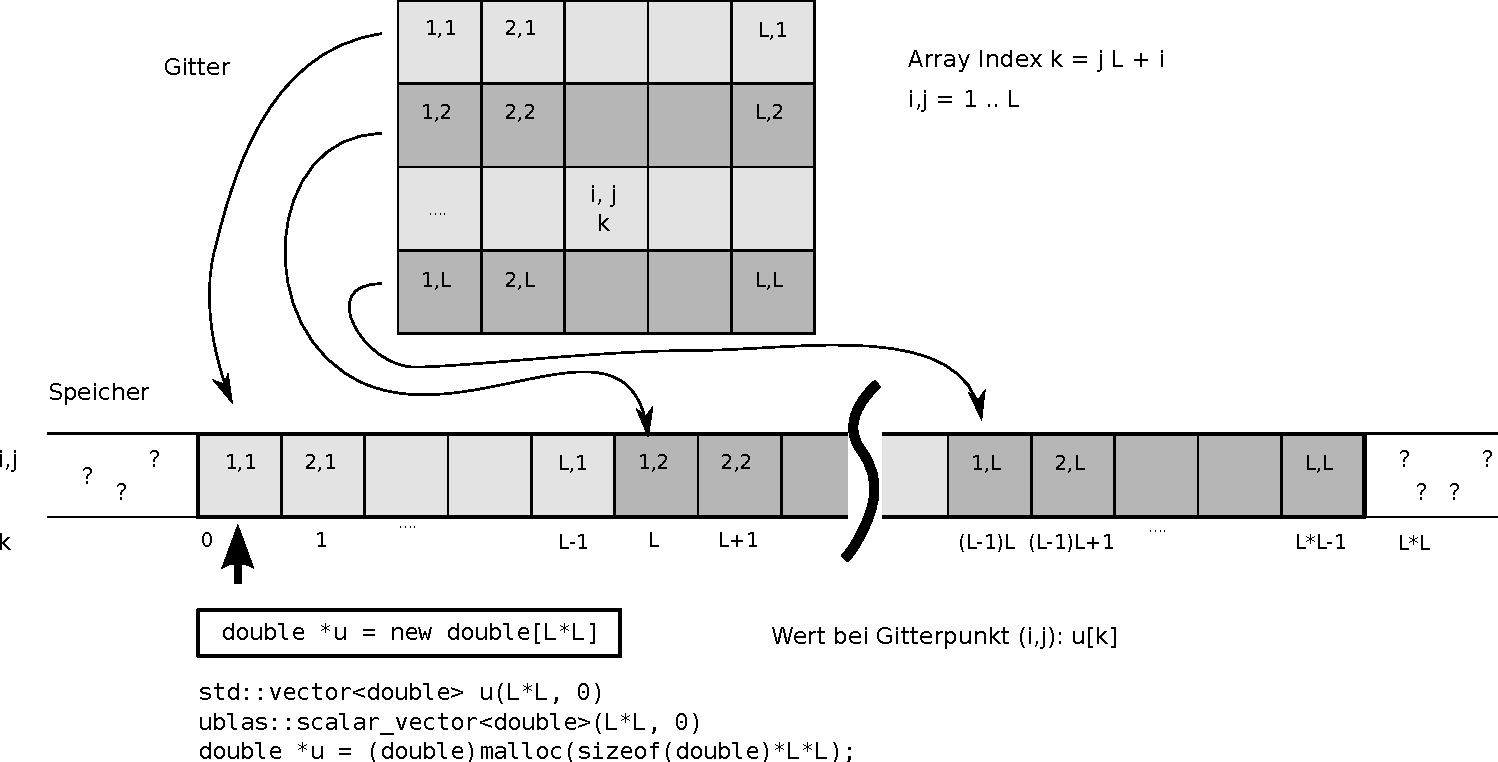
\includegraphics[scale=0.5]{img/speicher2.pdf}
\end{center}
\end{frame}



\begin{frame}
\frametitle{Volterra-Lotka - Numerische Lösung}
\begin{empheq}[box=\fbox]{align*}
%\begin{eqnarray}
u_{i,j}^{n+1}  &=& u_{i,j}^n + &\tau \left[ \delta_1 (\Delta_h u^n)_{i,j} + r u^n_{i,j} \left(1 - \frac{u^n_{i,j}}{w} \right) - p v^n_{i,j} \Psi(k u^n_{i,j}) \right] \\
v_{i,j}^{n+1}  &=& v_{i,j}^n + &\tau \left[ \delta_2 (\Delta_h v^n)_{i,j} + q v^n_{i,j} \Psi(k u^n_{i,j}) - s v^n_{i,j} \right]
%\end{eqnarray}
\end{empheq}
\newline\newline
\begin{itemize}
\item auf 2D Gitter wie vorhin! \\
\item $\frac{2 \delta_{1} \tau}{h^2}\leq 1$ und $\frac{2 \delta_{2} \tau}{h^2}\leq 1$
\end{itemize}
\end{frame}


% 
% \section{Vorbereitung}
% \begin{frame}{Vorbereitung}
% \textbf{Dateien}\\
% \begin{tabular}{ll}
% predator-prey-pde.cpp & C++ Quellcode\\
% compileit.sh & Shell-Script\\
% &\\
% diffusion & ausführbare Datei (zum testen)\\
% &\\
% run\_spiralwellen.sh & Shell-Script\\
% run\_gaussglocke.sh & Shell-Script\\
%  &\\
% plot.sh & Shell-Script\\
% plot.py & Python-Script\\
% makemovie.sh & Shell-Script
% \end{tabular}
% \end{frame}
% 
% \definecolor{lbcolor}{rgb}{0.9,0.9,0.9}
% \lstset{language=sh,backgroundcolor=\color{lbcolor}}
% 
% \begin{frame}[fragile]
% 
%   \frametitle{Vorbereitung}
% 
% \textbf{Kompilation} (compileit.sh)
% \small
% {
% \begin{lstlisting}
% g++ -O3 -o predator-prey-pde -lboost_program_options \
%   predator-prey-pde.cpp 
% \end{lstlisting}
% }
% 
% \textbf{Ausführen} (run\_spiralwellen.sh)
% \small
% {
% \begin{lstlisting}
% ./predator-prey-pde \
%   --mp-d2 1 \
%   --mp-q 1 \
%   --mp-s 0.5 \
%   --mp-k 5 \
%   --grid-size 200 \
%   --grid-spacing 1 \
%   --time-step 0.1 \
%   --max-time 200 \
%   --out-fn ./results/testrun \
%   --out-intervall 2
% \end{lstlisting}
% }
% \end{frame}
% 
% \begin{frame}[fragile]
% \textbf{Plots} (plot.sh)
% \begin{lstlisting}
% $sh ./plot.sh  datenfile.dat ausgabe.ps
% \end{lstlisting}
% startet gnuplot mit
% \lstset{language=gnuplot,backgroundcolor=\color{lbcolor}}
% \begin{lstlisting}
% set output '$dst'
% set terminal postscript color enhanced
% 
% set title '`basename $src`'
% set size square
% set xlabel 'x'
% set ylabel 'y'
% set cblabel '{/Symbol r}'
% 
% set pm3d map
% splot '$src' u 1:2:3 with pm3d title 'predators'
% splot '$src' u 1:2:4 with pm3d title 'prey'
% \end{lstlisting}
% \end{frame}
% 
% \lstset{language=sh,backgroundcolor=\color{lbcolor}}
% 
% \begin{frame}[fragile]
% \textbf{Bilderreihe}
% plot.py erzeugt png Bilder aus einer Reihe von .dat Dateien.
% \begin{lstlisting}
% $./plot.py ./results/testrun*.dat
% \end{lstlisting}
% \vspace{3pt}
% \textbf{Verwendung von mencoder} (makemovie.sh)
% \begin{lstlisting}
% mencoder \
%   "mf://*.png" -mf fps=15 \
%   -o ausgabevideo.avi \
%   -ovc lavc \
%   -lavcopts vcodec=mpeg4:vbitrate=8000
% \end{lstlisting}
% 
% \begin{lstlisting}
% $cd results
% $sh ../makemovie.sh
% $mplayer ausgabevideo.avi
% \end{lstlisting}
% \end{frame}


% \frame
% {
%   \frametitle{erste Testläufe}
% \textcolor{blue} {Erzeugen sie ein Video mithilfe von plot.py.}\\
% \textcolor{blue} {Erzeugen sie ein Bild mit plot.sh.}\newline\newline
% $$\frac{2 D \Delta t}{\left(\Delta x\right)^2}\leq 1$$
% \textcolor{blue} {Wie sehen die numerischen Lösungen aus, wenn dieses Kriterium nicht erfüllt ist?}
% }



\section{C++}

\begin{frame}{Scope of Variables}
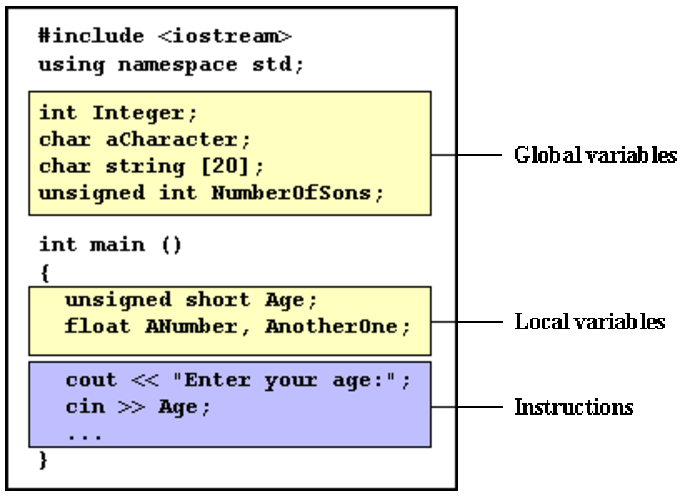
\includegraphics[height=7cm]{img/scope_of_variables.pdf} 
\end{frame}

\begin{frame}[fragile]
  \frametitle{if}
  \definecolor{lbcolor}{rgb}{0.9,0.9,0.9}
  \lstset{language=C++,backgroundcolor=\color{lbcolor}}
  %\lstinputlisting{predator-prey-ode.cpp}
Verzweigungen
\begin{lstlisting}
if (Ausdruck) Anweisung;
\end{lstlisting}
oder
\begin{lstlisting}
if (Ausdruck)
{
  Anweisung_1;
  Anweisung_2;
}
else
  Anweisung_3;
\end{lstlisting}
\end{frame}

\begin{frame}[fragile]{switch}
Verzweigungen mit ``switch''
\begin{lstlisting}
switch (Zeichen)
{
  case 1: Anweisung_1; break;
  case 2: Anweisung_2; break;
  ...
  default:  Anweisung; break;
}
\end{lstlisting}
\end{frame}

\begin{frame}[fragile]
  \frametitle{for}
  \definecolor{lbcolor}{rgb}{0.9,0.9,0.9}
  \lstset{language=C++,backgroundcolor=\color{lbcolor}}
  %\lstinputlisting{predator-prey-ode.cpp}

Läuft bis Ausdruck ``false'' ergibt.
\begin{lstlisting}
for (Initialisierung; Ausdruck; Inkrement)
{
  Anweisung_1;
  Anweisung_2;
  ...
}
\end{lstlisting}

Beispiel:
\begin{lstlisting}
for (int i=0; i<n ;i++)
    a[i] += b * c[i];
\end{lstlisting}
Die Zählvariable i kann in der Initialisierung deklariert werden.

\end{frame}

\begin{frame}[fragile]
  \frametitle{while und do $\ldots$ while}
  \definecolor{lbcolor}{rgb}{0.9,0.9,0.9}
  \lstset{language=C++,backgroundcolor=\color{lbcolor}}
  %\lstinputlisting{predator-prey-ode.cpp}
\begin{lstlisting}
while (Ausdruck)
{
  Anweisung_1;
  Anweisung_2;
}
\end{lstlisting}

\begin{lstlisting}
do
{
  Anweisung_1;
  Anweisung_2;
}
while (Ausdruck)
\end{lstlisting}

\begin{lstlisting}
break beendet den ganzen Schleifendurchlauf
\end{lstlisting}
\begin{lstlisting}
continue beendet den aktuellen Schleifendurchlauf
\end{lstlisting}

\end{frame}

\begin{frame}[fragile]
  \frametitle{Funktionen}
  \definecolor{lbcolor}{rgb}{0.9,0.9,0.9}
  \lstset{language=C++,backgroundcolor=\color{lbcolor}}
  %\lstinputlisting{predator-prey-ode.cpp}
\begin{lstlisting}
void DoSomething()
{
  Anweisungen;
}
\end{lstlisting}
\begin{lstlisting}
double Addition(double a, double b)
{
  return a+b;
}

\end{lstlisting}
\begin{lstlisting}
void Addition(double &a, const double &b)
{
  a += b;
}
\end{lstlisting}
\end{frame}



\begin{frame}[fragile]
  \frametitle{Templates}
  \definecolor{lbcolor}{rgb}{0.9,0.9,0.9}
  \lstset{language=C++,backgroundcolor=\color{lbcolor}}
  \begin{lstlisting}
template<class T>
T Addition(T a, T b)
{
  return a+b;
}

double x = Addition<double>(1., 2.);
int    i = Addition<int>(1,2);
  \end{lstlisting}

  \begin{lstlisting}
template<class T>
class PimpedArray
{
  T *data;
  ...
};

PimpedArray<double> doubleArray;
PimpedArray<int>    intArray;
  \end{lstlisting}
\end{frame}


\begin{frame}[fragile]
  \frametitle{Das Assert Makro}
  \definecolor{lbcolor}{rgb}{0.9,0.9,0.9}
  \lstset{language=C++,backgroundcolor=\color{lbcolor}}
  \begin{lstlisting}    
    #include <assert.h>
    Assert(expression); 
    // Programabbruch mit Fehlermeldung 
    // falls expression==false
    
    // Definiere NDEBUG um das Makro abzuschalten
  \end{lstlisting}
\end{frame}


\begin{frame}
Referenzen
\begin{itemize}
\item \url{www.cplusplus.com}
\item \url{www.cplusplus.com/doc/tutorial}
\item Boost Library \url{www.boost.org}
\item The GNU Project Debugger \url{www.gnu.org/software/gdb}
\end{itemize}
Zusätzliche Referenzen
\begin{itemize}
\item \url{www.python.org} (plot.py ist noch für python 2.7)
\item \url{docs.python.org/2/}
\item \url{rgruet.free.fr/PQR27/PQR2.7.html} (Python Schnellreferenz)
\item \url{matplotlib.org/}
%\item Eigen (alternative zu-und imo besser als ublas) \url{http://eigen.tuxfamily.org}
\end{itemize}
\end{frame}
%http://www.cplusplus.com/reference/cassert/assert/

\end{document}
